
%(BEGIN_QUESTION)
% Copyright 2010, Tony R. Kuphaldt, released under the Creative Commons Attribution License (v 1.0)
% This means you may do almost anything with this work of mine, so long as you give me proper credit

The following ``bubbler'' level measurement system has a problem.  It registers zero level at all times, no matter what the actual liquid level is in the tank.  Inspecting the rotameter, you see it does register a continuing flow of purge air:

$$\includegraphics[width=15.5cm]{i04680x01.eps}$$

Identify the likelihood of each specified fault for this circuit.  Consider each fault one at a time (i.e. no coincidental faults), determining whether or not each fault could independently account for {\it all} measurements and symptoms in this circuit.

% No blank lines allowed between lines of an \halign structure!
% I use comments (%) instead, so that TeX doesn't choke.

$$\vbox{\offinterlineskip
\halign{\strut
\vrule \quad\hfil # \ \hfil & 
\vrule \quad\hfil # \ \hfil & 
\vrule \quad\hfil # \ \hfil \vrule \cr
\noalign{\hrule}
%
% First row
{\bf Fault} & {\bf Possible} & {\bf Impossible} \cr
%
\noalign{\hrule}
%
% Another row
Leak in dip tube above liquid level &  &  \cr
%
\noalign{\hrule}
%
% Another row
Valve $V_1$ closed &  &  \cr
%
\noalign{\hrule}
%
% Another row
Valve $V_2$ closed &  &  \cr
%
\noalign{\hrule}
%
% Another row
Valve $V_3$ closed &  &  \cr
%
\noalign{\hrule}
%
% Another row
Valve $V_4$ closed &  &  \cr
%
\noalign{\hrule}
%
% Another row
Regulator mis-adjusted &  &  \cr
%
\noalign{\hrule}
%
% Another row
Dip tube plugged &  &  \cr
%
\noalign{\hrule}
%
% Another row
Air supply dead &  &  \cr
%
\noalign{\hrule}
%
% Another row
Leak in dip tube below liquid surface &  &  \cr
%
\noalign{\hrule}
} % End of \halign 
}$$ % End of \vbox

Finally, identify the {\it next} diagnostic test or measurement you would make on this system.  Explain how the result(s) of this next test or measurement help further identify the location and/or nature of the fault.

\underbar{file i04680}
%(END_QUESTION)





%(BEGIN_ANSWER)


%(END_ANSWER)





%(BEGIN_NOTES)

% No blank lines allowed between lines of an \halign structure!
% I use comments (%) instead, so that TeX doesn't choke.

$$\vbox{\offinterlineskip
\halign{\strut
\vrule \quad\hfil # \ \hfil & 
\vrule \quad\hfil # \ \hfil & 
\vrule \quad\hfil # \ \hfil \vrule \cr
\noalign{\hrule}
%
% First row
{\bf Fault} & {\bf Possible} & {\bf Impossible} \cr
%
\noalign{\hrule}
%
% Another row
Leak in dip tube above liquid level & $\surd$ &  \cr
%
\noalign{\hrule}
%
% Another row
Valve $V_1$ closed &  & $\surd$ \cr
%
\noalign{\hrule}
%
% Another row
Valve $V_2$ closed & $\surd$ &  \cr
%
\noalign{\hrule}
%
% Another row
Valve $V_3$ closed &  & $\surd$ \cr
%
\noalign{\hrule}
%
% Another row
Valve $V_4$ closed & ? & \cr
%
\noalign{\hrule}
%
% Another row
Regulator mis-adjusted &  & $\surd$ \cr
%
\noalign{\hrule}
%
% Another row
Dip tube plugged &  & $\surd$ \cr
%
\noalign{\hrule}
%
% Another row
Air supply dead &  & $\surd$ \cr
%
\noalign{\hrule}
%
% Another row
Leak in dip tube below liquid surface &  & $\surd$ \cr
%
\noalign{\hrule}
} % End of \halign 
}$$ % End of \vbox

Valve $V_4$ being left closed is a possibility only if the equalizing valve $V_3$ were to leak over time, and the process liquid level remains absolutely constant.  Over time, the transmitter's DP will approach zero (since the ``L'' side cannot vent to atmosphere), resulting in a zero indication.  However, since one could argue a leaking equalizing valve is really a {\it second} fault and therefore should not be considered according to the rules of this fault analysis, its ``possible'' status is questionable.

\vskip 10pt

A good ``next test'' would be to check the positions of the manifold valves, to ensure both block valves are open and the equalizing valve is shut.  Another test would be to completely shut restrictor valve $V_1$ and see if the reading changes at all.





\vskip 20pt \vbox{\hrule \hbox{\strut \vrule{} {\bf Virtual Troubleshooting} \vrule} \hrule}

This question is a good candidate for a ``Virtual Troubleshooting'' exercise.  Presenting the diagram to students, you first imagine in your own mind a particular fault in the system.  Then, you present one or more symptoms of that fault (something noticeable by an operator or other user of the system).  Students then propose various diagnostic tests to perform on this system to identify the nature and location of the fault, as though they were technicians trying to troubleshoot the problem.  Your job is to tell them what the result(s) would be for each of the proposed diagnostic tests, documenting those results where all the students can see.

During and after the exercise, it is good to ask students follow-up questions such as:

\begin{itemize}
\item{} What does the result of the last diagnostic test tell you about the fault?
\item{} Suppose the results of the last diagnostic test were different.  What then would that result tell you about the fault?
\item{} Is the last diagnostic test the best one we could do?
\item{} What would be the ideal order of tests, to diagnose the problem in as few steps as possible?
\end{itemize}


%INDEX% Measurement, level: troubleshooting

%(END_NOTES)

